\documentclass{article}
\usepackage{amsmath}
\usepackage{amssymb}
\usepackage[svgnames]{xcolor}
\usepackage{graphicx}
\usepackage{enumitem}
\usepackage{multicol}
\usepackage{bbm}

\title{Computer Graphics: Assignment 08} % Title

\author{Lina Gundelwein, Letitia Parcalabescu, Anushalakshmi Manila} % Author name

\date{\today} % Date for the report

\begin{document}

\maketitle 

\section{Clipping}
\begin{figure}[htb]
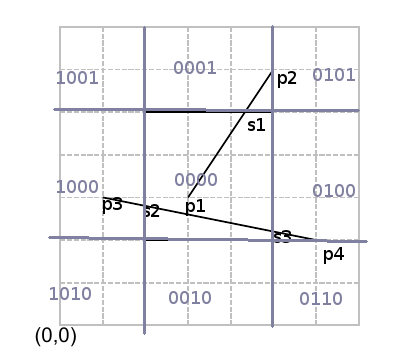
\includegraphics[scale=0.5]{01}
\end{figure}
First line
\begin{itemize}
\item Outcode($P_1$) $\vee$ Outcode($P_2$) $\neq 0$ $\rightarrow$ no trivial accept
\item Outcode($P_1$) $\wedge$ Outcode($P_2$)$ == 0$ $\rightarrow$ no trivial reject
\item Calculate $S_1$
\item Outcode($P_1$) $\vee$ Outcode($S_1$) $== 0$ $\rightarrow$ trivial accept
\end{itemize}
Second line
\begin{itemize}
\item Outcode($P_3$) $\vee$ Outcode($P_4$) $\neq 0$ $\rightarrow$ no trivial accept
\item Outcode($P_3$) $\wedge$ Outcode($P_4$)$ == 0$ $\rightarrow$ no trivial reject
\item Calculate $S_2$
\item Outcode($P_4$) $\vee$ Outcode($S_2$) $\neq 0$ $\rightarrow$ no trivial accept
\item Outcode($P_4$) $\vee$ Outcode($S_2$) $== 0$ $\rightarrow$ no trivial reject
\item Calculate $S_3$
\item Outcode($S_3$) $\vee$ Outcode($S_2$) $==0$ $\rightarrow$ trivial accept

\end{itemize}
\section{Polygon Clipping}
\begin{itemize}
\item n+1
\item n+
\end{itemize}

\section{Sutherland Hodgman Algorithm}
\begin{itemize}
\item Clip top
\begin{itemize}
\item $P_1P_2 \rightarrow P_2$
\item $P_2P_3 \rightarrow S_1 = (0.7,1.0)$
\item $P_3P_4 \rightarrow S_2 = (-0.5,1.0), P_4$
\item $P_4P_1 \rightarrow P_1$
\end{itemize}
\item Clip bottom
\begin{itemize}
\item $P_1P_2 \rightarrow P_2$
\item $P_2S_1 \rightarrow S_1$
\item $S_1S_2 \rightarrow S_2$
\item $S_2P_4 \rightarrow P_4$
\item $P_4P_1 \rightarrow P_1$
\end{itemize}
\item Clip right
\begin{itemize}
\item $P_1P_2 \rightarrow S_3 = (1.0,-0.875)$
\item $P_2S_1 \rightarrow S_4 = (1.0,0.25), S_1$
\item $S_1S_2 \rightarrow S_2$
\item $S_2P_4 \rightarrow P_4$
\item $P_4P_1 \rightarrow P_1$
\end{itemize}
\item Clip left
\begin{itemize}
\item $P_1S_3 \rightarrow S_3$
\item $S_3S_4 \rightarrow S_4$
\item $S_4S_1 \rightarrow S_1$
\item $S_1S_2 \rightarrow S_2$
\item $S_2P_4 \rightarrow S_5 = (-1.0,0.75)$
\item $P_4P_1 \rightarrow S_6 = (-1.0,0), P_1$
\end{itemize}
\end{itemize}
$\Rightarrow$ clipped polygon: $S_3, S_4,S_1,S_2, S_5, S_6, P_1$
\end{document}